\documentclass[crop, tikz]{standalone}
\usepackage{tikz}

\usetikzlibrary{positioning}

\begin{document}
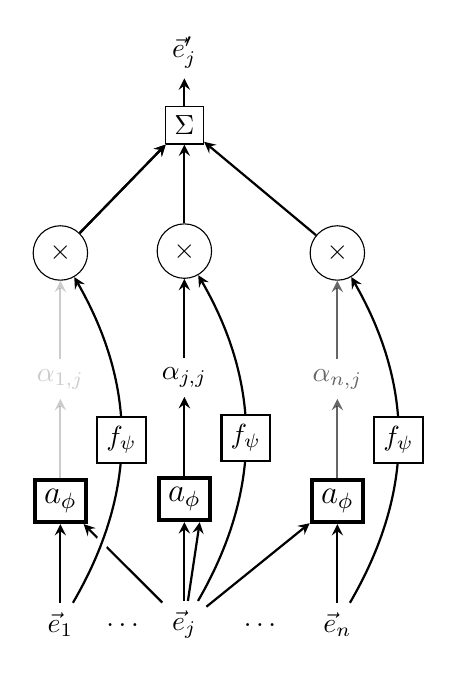
\begin{tikzpicture}

	\node (X1) {$\vec{e}_{1}$};

	\node[rectangle, right= 0.5em of X1] (x_dots_1) {$\dots$};

	\node[right=0.5em of x_dots_1] (Xj) {$\vec{e}_{j}$};

	\node[rectangle, right= 1em of Xj] (x_dots_2) {$\dots$};

	\node[right=1em of x_dots_2] (Xn) {$\vec{e}_{n}$};

	\node[rectangle, draw, ultra thick, above=of X1] (attn1) {\large $a_\phi$};

	\node[rectangle, draw, ultra thick, above=of Xj] (attnj) {\large $a_\phi$};

	\node[rectangle, draw, ultra thick, above=of Xn] (attnn) {\large $a_\phi$};


	\draw[-stealth, thick] (X1) -- (attn1);
	\draw[-stealth, thick] (Xj) -- (attn1);

	\draw[-stealth, thick] (Xj) -- (attnj);
	\draw[-stealth, thick] ([xshift=3em]Xj) -- (attnj);
	
	\draw[-stealth, thick] (Xj) -- (attnn);
	\draw[-stealth, thick] (Xn) -- (attnn);
	
	\node[above= of attn1, opacity=0.2] (alpha1j) {$\alpha_{1,j}$};
	\node[above= of attnj, opacity=1] (alphajj) {$\alpha_{j,j}$};
	\node[above= of attnn, opacity=0.6] (alphanj) {$\alpha_{n,j}$};
	
	\node[circle, draw, above=of alpha1j] (times1) {$\times$};
	\node[circle, draw, above=of alphajj] (timesj) {$\times$};
	\node[circle, draw, above=of alphanj] (timesn) {$\times$};
	
	\node[rectangle, draw, above=of timesj] (sum) {$\Sigma$};

	\node[above=1em of sum] (x_tprim) {$\vec{e}_j'$};

	\draw[-stealth, line width=1.5mm, white] (attn1) -- (alpha1j);
	\draw[-stealth, thick, opacity=0.2] (attn1) -- (alpha1j);
	\draw[-stealth, line width=1.5mm, white] (attnj) -- (alphajj);
	\draw[-stealth, thick, opacity=1] (attnj) -- (alphajj);
	\draw[-stealth, line width=1.5mm, white] (attnn) -- (alphanj);
	\draw[-stealth, thick, opacity=0.6] (attnn) -- (alphanj);
	
	\draw[-stealth, white, line width=1.5mm] (X1) edge[bend right=30] (times1);
	\draw[-stealth, thick] (X1) edge[bend right=30] node[rectangle, draw, fill=white, midway] {$f_\psi$} (times1);
	\draw[-stealth, white, line width=1.5mm] (Xj) edge[bend right=30] (timesj);
	\draw[-stealth, thick] (Xj) edge[bend right=30] node[rectangle, draw, fill=white, midway] {$f_\psi$} (timesj);
	\draw[-stealth, thick] (Xn) edge[bend right=30] node[rectangle, draw, fill=white, midway] {$f_\psi$} (timesn);

	\draw[-, line width=1.5mm, white] (times1) -- (sum);
	\draw[-stealth, thick] (times1) -- (sum);
	\draw[-, line width=1.5mm, white] (timesj) -- (sum);
	\draw[-stealth, thick] (timesj) -- (sum);
	\draw[-stealth, thick] (timesn) -- (sum);
	\draw[-stealth, thick] (times1) -- (sum);
		
	\draw[-stealth, line width=1.5mm, white] (alpha1j) -- (times1);
	\draw[-stealth, thick, opacity=0.2] (alpha1j) -- (times1);
	\draw[-stealth, line width=1.5mm, white] (alphajj) -- (timesj);
	\draw[-stealth, thick, opacity=1] (alphajj) -- (timesj);
	\draw[-stealth, line width=1.5mm, white] (alphanj) -- (timesn);
	\draw[-stealth, thick, opacity=0.6] (alphanj) -- (timesn);

	\draw[-stealth, thick] (sum) -- (x_tprim);

\end{tikzpicture}
\end{document}